% ---------------------------------------------------------------------------
% Author guideline and sample document for EG publication using LaTeX2e input
% D.Fellner, v1.15, Dec 14, 2018

\documentclass{egpubl}
 
% --- for  Annual CONFERENCE
% \ConferenceSubmission   % uncomment for Conference submission
% \ConferencePaper        % uncomment for (final) Conference Paper
% \STAR                   % uncomment for STAR contribution
% \Tutorial               % uncomment for Tutorial contribution
% \ShortPresentation      % uncomment for (final) Short Conference Presentation
% \Areas                  % uncomment for Areas contribution
% \MedicalPrize           % uncomment for Medical Prize contribution
% \Education              % uncomment for Education contribution
% \Poster                 % uncomment for Poster contribution
% \DC                     % uncomment for Doctoral Consortium
%
% --- for  CGF Journal
\JournalSubmission    % uncomment for submission to Computer Graphics Forum
%\JournalPaper         % uncomment for final version of Journal Paper
%
% --- for  CGF Journal: special issue
% \SpecialIssueSubmission    % uncomment for submission to , special issue
% \SpecialIssuePaper         % uncomment for final version of Computer Graphics Forum, special issue
%                          % EuroVis, SGP, Rendering, PG
% --- for  EG Workshop Proceedings
% \WsSubmission      % uncomment for submission to EG Workshop
% \WsPaper           % uncomment for final version of EG Workshop contribution
% \WsSubmissionJoint % for joint events, for example ICAT-EGVE
% \WsPaperJoint      % for joint events, for example ICAT-EGVE
% \Expressive        % for SBIM, CAe, NPAR
% \DigitalHeritagePaper
% \PaperL2P          % for events EG only asks for License to Publish

% --- for EuroVis 
% for full papers use \SpecialIssuePaper
% \STAREurovis   % for EuroVis additional material 
% \EuroVisPoster % for EuroVis additional material 
% \EuroVisShort  % for EuroVis additional material

% !! *please* don't change anything above
% !! unless you REALLY know what you are doing
% ------------------------------------------------------------------------
\usepackage[T1]{fontenc}
\usepackage{dfadobe}  

%\usepackage{cite}  % comment out for biblatex with backend=biber
% ---------------------------
\biberVersion
\BibtexOrBiblatex
\usepackage[backend=biber,bibstyle=EG,citestyle=alphabetic,backref=true]{biblatex} 
\addbibresource{test.bib}
% ---------------------------  
\electronicVersion
\PrintedOrElectronic
% for including postscript figures
% mind: package option 'draft' will replace PS figure by a filename within a frame
\ifpdf \usepackage[pdftex]{graphicx} \pdfcompresslevel=9
\else \usepackage[dvips]{graphicx} \fi

\usepackage{egweblnk} 
% end of prologue
\usepackage{amsmath}
\usepackage{bbold}
\usepackage{amsmath}
\usepackage{amsfonts}
\usepackage{amssymb}
\usepackage{graphicx}
\usepackage{color}
\usepackage{colortbl}
\usepackage{multirow}
\usepackage{subcaption}
\usepackage{hhline}
\usepackage{url}
\usepackage{algorithm}
\graphicspath{{./images/}}
\usepackage{algpseudocode}
\usepackage{nicefrac}
\usepackage{mathtools}
\usepackage{tabularx}
\usepackage{mathbbol}
\DeclareMathOperator*{\sgn}{sgn}
\DeclareMathOperator*{\argmax}{arg\,max}
\DeclareMathOperator*{\argmin}{arg\,min}
\newcommand{\prob}[2]{\mathbf{#1}_{#2} \otimes \mathbf{#1}_{#2} \otimes \mathbf{#1}_{#2}
\otimes \mathbf{#1}_{#2}}
\def\cT {\mathcal{T}} 
\def\cR {\mathcal{R}}
\def\cO {\mathcal{O}}  
\usepackage{booktabs} % http://ctan.org/pkg/booktabs
\usepackage{xparse}
\NewDocumentCommand{\rot}{O{45} O{1em} m}{\makebox[#2][l]{\rotatebox{#1}{#3}}}%
\definecolor{lightgreen}{RGB}{144,238,144}
\definecolor{lightred}{RGB}{255,204,203}
%\author[Submission ID 1025]
%{\parbox{\textwidth}{\centering Submission ID 1025}\\{\parbox{\textwidth}{\centering ***}}}
 \author[J.~Grün et al.]
{\parbox{\textwidth}{\centering J.~Gruen\orcid{0000-0002-9154-3929}, G.~van der Voort\orcid{0000-0003-1008-9160}, and T.~Schultz\orcid{0000-0002-1200-7248}
	}
	\\
	{\parbox{\textwidth}{\centering University of Bonn, Bonn, Germany}}
}
\title{Model Averaging and Bootstrap Consensus Based Uncertainty Reduction in Diffusion MRI Tractography}

\begin{document}
\maketitle
\begin{abstract}
  
  Diffusion Magnetic Resonance Imaging (dMRI) tractography has the
  unique ability to reconstruct major white matter tracts
  non-invasively and is therefore widely used in neurosurgical
  planning and neuroscience. In this work, we reduce two sources of
  uncertainty within the tractography pipeline. The first one is the
  model uncertainty that arises in crossing fiber tractography, from
  having to estimate the number of relevant fiber compartments in each
  voxel. The second one is the data uncertainty that arises from
  measurement noise. We propose a mathematical framework to estimate
  model uncertainty, and we reduce this type of uncertainty with a
  model averaging approach that combines the fiber direction estimates
  from all candidate models, weighted by the posterior probability of
  the respective model. We use bootstrapping to estimate data
  uncertainty, and consolidate the fiber direction estimates from all
  bootstraps into a consensus model. We observe that a traditional
  model selection strategy frequently selects different models in
  different bootstraps. In this sense, the bootstrap consensus also
  reduces model uncertainty. Either approach increases the accuracy of
  crossing fiber tractography in multiple subjects, and combining them
  provides a small additional benefit.
  
  \textbf{Keywords:} diffusion MRI, tractography, uncertainty, model averaging, bootstrapping
%-------------------------------------------------------------------------
%  ACM CCS 1998
%  (see https://www.acm.org/publications/computing-classification-system/1998)
% \begin{classification} % according to https://www.acm.org/publications/computing-classification-system/1998
% \CCScat{Computer Graphics}{I.3.3}{Picture/Image Generation}{Line and curve generation}
% \end{classification}
%-------------------------------------------------------------------------
%  ACM CCS 2012
%   (see https://www.acm.org/publications/class-2012)
%The tool at \url{http://dl.acm.org/ccs.cfm} can be used to generate
% CCS codes.
%Example:
\begin{CCSXML}
<ccs2012>
   <concept>
       <concept_id>10010405.10010444</concept_id>
       <concept_desc>Applied computing~Life and medical sciences</concept_desc>
       <concept_significance>500</concept_significance>
       </concept>
   <concept>
       <concept_id>10002950.10003648.10003671</concept_id>
       <concept_desc>Mathematics of computing~Probabilistic algorithms</concept_desc>
       <concept_significance>400</concept_significance>
       </concept>
   <concept>
       <concept_id>10003120.10003145.10003146</concept_id>
       <concept_desc>Human-centered computing~Visualization techniques</concept_desc>
       <concept_significance>400</concept_significance>
       </concept>
 </ccs2012>
\end{CCSXML}

\ccsdesc[500]{Applied computing~Life and medical sciences}
\ccsdesc[400]{Mathematics of computing~Probabilistic algorithms}
\ccsdesc[400]{Human-centered computing~Visualization techniques}

\printccsdesc   
\end{abstract}  

\section{Introduction}
Diffusion Magnetic Resonance Imaging (dMRI) \cite{LeBihan:1986} is a
non-invasive vital imaging method for the human brain. It particularly has the
unique ability to get insights into major white matter tracts within the human
brain and can
reconstruct large parts of the white matter tracts, using tractography algorithms. dMRI is based on
inferring the fiber tracts using the Brownian motion of water molecules. Since
the fiber tracts impede the water movement it will move along the fiber tracts
rather than orthogonal to it. 
This unique ability of fiber tracking makes dMRI an important feature for large
scientific studies \cite{Sotiropoulos:2013, Tobisch:2018Frontiers} as well as surgery planning \cite{Yang:2021}.

The process of obtaining tractograms is not trivial at all and contains many
pitfalls. The most popular and widely used approaches recover the local
orientation of fiber tracts from dMRI measurements. This is an ill
conditioned inverse problem \cite{TOURNIER20071459}. Earlier approaches, like
diffusion tensor imaging \cite{BASSER1994247}
were just able to recover a single direction per voxel, which is not sufficient
to recover more complex geometries like fibre crossing, kissing and bending.
Newer approaches rely on high angular resolution imaging (HARDI). Within the
last decade there have been many methods invented to compute multiple local orientations
from raw diffusion data, including the
ball-and-stick model \cite{BEHRENS2007144}, and the low-rank approximation of high order fODF tensors
\cite{lowrank, Ankele:CARS2017}.

Within our last work we have evaluated the influence of model uncertainty in
the low-rank approximation in a systematical way. To be more precise, the fiber
count has to be set a priori to apply the low-rank approximation. This is a
crucial step, since setting the number to low will miss relevant directions and
setting the number to high will introduce wrong directions which makes the
tracking process even more challenging. Further the remaining directions are
more error-prone, if the number is not set correctly. 
Therefore, we estimated the number of fibers with the help of a Bayesian model and
created a selection model from these estimations. To improve the precision of
the local direction fields
further, we proposed a novel averaging model, which fuses all the different
low-rank approximations into a new model and therefore, reduces this source of
uncertainty even further.
Using a probabilistic fiber tracking model, it has been shown that fiber
tracking within the newly proposed models is more robust and results in
better reconstructions compared to fiber tracking within a state of the art
 $8$th constrained spherical deconvolution model.

With the increasing complexity of scanner protocols and the resulting more
complex models also the sensitivity to measurement noise increases. Within this work
we will systematically investigate the influence of noise to the generated
models. We use a wild bootstrapping approach, which has been
successfully applied to dMRI in many cases \cite{Jones:2008}. Instead of
calculating a fiber distribution to visualize uncertainty, we proceed in
another way and evaluate the impact of noise to the average, selection, and
low-rank model.

We are using the newly derived quantification of measurement uncertainty to the
direction fields to generate a novel consensus bootstrap
model, which fuses all the bootstrap information into a single model. This new
approach is then compared to the previously derived models as well as the
rank-$3$ model. We conclude that the
impact on crossing fiber tractography depends highly on the model. While the
improvement in the selection model is huge, the improvement of the
average model is not large. 

In Section \ref{related} we will introduce some related work which will help the
reader to put our work into the right context. This is followed in Section \ref{background} by an
explanation of the model on which our approach is based.

\section{Related Work}\label{sec:related}
\added{There is a substantial body of literature on algorithms for diffusion MRI tractography \cite{Jeurissen:2018}, and many of them were first introduced in visualization venues \cite{Weinstein:1999,Zhang:2003,Hlawitschka:2005,lowrank}. The visualization and reduction of various sources of uncertainty in the tractography pipeline has been a more recent focus of interest \cite{Brecheisen:2009,Brecheisen:2013,Schultz:SciVisBook2014,Wiens:2014,Siddiqui:2021,Gruen:2021}. These sources}
%
can broadly be categorised into measurement uncertainty,
model uncertainty, parameter uncertainty, and partial voluming \cite{Schultz:SciVisBook2014, Schultz:NBM2018, Gillmann:STAR2021}.

The impact of measurement
uncertainty on the dMRI pipeline has been widely estimated with probabilistic tractography, based on Bayesian modeling \cite{BEHRENS2007144} or bootstrapping \cite{Jones:2008}. Instead of a single streamline per seed, this recovers distributions,
which can be visualized using hyperstreamlines \cite{Jones:2005b,Jeurissen:2012, Wiens:2014}
or confidence intervals \cite{Brecheisen:2013,Siddiqui:2021}. Our work explores a different use of bootstrapping, which performs uncertainty reduction by consolidating estimates from all bootstraps into a single consensus that is used for tracking.

We refer to model uncertainty as the uncertainty which arises from the choice
between several mathematical models to extract directions from the dMRI data
\cite{Schultz:SciVisBook2014}. There exists a wide range of models to estimate
fiber directions \cite{Panagiotaki:2012}, and they might lead to different
results. \added{Comparative visualization has been used to investigate such differences \cite{Vos:2013,Schultz:EuroVis2013}.} There is no generally preferable model, since the suitability depends  on the dMRI acquisition scheme, as well as on
the anatomical location \cite{Bretthorst:2004,Freidlin:2007}. Our current work significantly extends a recent workshop paper that investigated a special case of model uncertainty, focusing on the aspect of selecting a suitable voxel-specific fiber direction count \cite{Gruen:2021}. 

Another type of uncertainty arises from parameter choices within the tracking algorithm itself, which for example control branching to reproduce fiber spread, or the termination of individual streamlines. Brecheisen et al.\ proposed a visual tool to systematically explore the impact of such parameters
\cite{Brecheisen:2009}. \added{Since optimal settings depend on the specific tract, Takemura et al.\ developed an ensembling approach that selects streamlines from candidates that have been generated with different algorithms and parameters \cite{Takemura:2016}.}

Finally, the partial volume effect is
an important source of uncertainty in dMRI. It arises from the fact that the diameter of individual axons is orders of magnitude smaller than the spatial resolution of dMRI. Even when correctly accounting for cases in which axons cross \cite{Alexander:2001,BEHRENS2007144} or spread \cite{Kaden:2007} at a voxel level, situations in which two distinct tracts become locally aligned pose a fundamental difficulty for finding their correct continuation. This has been referred to as the bottleneck issue \cite{Schilling:2022}, and it contributes to the fact that, even though dMRI tractography quite successfully localizes true tracts in individual subjects, it tends to produce many false positives \cite{MaierHein:2017}. These have to be eliminated using prior anatomical knowledge, which can be represented implicitly using machine learning \cite{WASSERTHAL2018239}, or explicitly by defining regions of interest to include or exclude streamlines \cite{Wakana:2007}. Our work employs the latter approach.

%%% Local Variables:
%%% mode: latex
%%% TeX-master: "../main"
%%% End:

\section{Background}
\begin{itemize}
	\item Introduce spherical deconvolution since it is the basis for
		bootstrapping. 

\end{itemize}
Spherical deconvolution is based on solving the linear least square problem 
\begin{align}
	\argmin_{\mathcal{T}} \| M \mathcal{T} - S \|^2,
	\label{eq:sd-min}
\end{align}
where 
$M$ denotes the convolution matrix, $S$ the signal and $\mathcal{T}$ the fODF.
Earlier approaches expressed the fODF as spherical function and imposed a
non-negativity constraint to Eq. (\ref{eq:sd-min}). The constrained is justified by
the fact, that the fODF should represent the fiber fraction in any given
direction, which is clearly positive. 
Newer approaches express the fODF as symmetric fourth order tensor and apply a
H-psd constrained, which implies non-negativity but not vice versa. It has been
demonstrated, that latter expression increases the angular resolution. 

From the symmetric fourth order fODF $\mathcal{T}f$ peaks are extracted via a rank-$r$
approximation 
\begin{align}
	\mathcal{T}^{\left( r \right)} = \sum_{i=1}^r \lambda_i \mathbf{v}_i
	\otimes \mathbf{v}_i \otimes \mathbf{v}_i \otimes \mathbf{v}_i, 
	\label{eq:low-rank}
\end{align}
where the scalar $\lambda_i$ represents the volume fraction of the $i$th fiber,
the unit vector $\mathbf{v}_i \in \mathbb{R}^3$ its direction and $\otimes$ the
outer product. The approximation is done by calculating 
\[ \argmin_{\lambda_1, \dots , \lambda_r , \mathbf{v}_1, \dots , \mathbf{v}_r}
\| \mathcal{T} - \mathcal{T}^{\left( r \right)} \|_F, \]
where $\| \cdot \|_F$ denotes the Frobenius norm. In case of fiber crossings the
used methods have a highly reduced angular error, as it was demonstrated in XY,
compared to peak extraction, which is applied to spherical function fODFs. 

\begin{itemize}
	\item Hier noch beschreiben, dass CSD schon measurement noise reduziert. 
	\item Vielleicht das ganze noch umsortieren. Gerade etwas durcheinander. 
\end{itemize}

\section{Averaging and Selection Model}\label{sec:Models}

Within our work we have proposed a probabilistic framework
to quantify the posterior probability with which different potential fiber values
are suitable given a local fODF.
Using these information is especially for the low-rank approximation important,
since a wrong assumption on the number of fibers in a local voxel introduces new
fiber directions or misses important fibre directions. Which then leads to false
positive or false negatives. Further, the fibers are not independent of each
other, i.e. missing the correct number will also introduce an error to the
fibers.

\subsection{Bayesian Model Comparison}
We use a Bayesian model comparison approach, i.e. we are interested in the
posterior probability $p \left( \mathcal{H}_r \mid \mathcal{T} \right)$, where
$\mathcal{H}_r$ denotes the hypothesis that rank $r$ is the optimal rank to
extract $r$ fibers from a given fODF $\mathcal{T}$. Using Bayes' theorem of
conditional probability, the posterior probability can be rewritten as
\begin{align}
	p \left( \mathcal{H}_r \mid \mathcal{T} \right) \propto p \left(
		\mathcal{T} \mid \mathcal{H}_r 
	\right) p \left(  \mathcal{H}_r \right), 
	\label{eq:Bayes}
\end{align}
where $p \left(  \mathcal{H}_r \right)$ is our prior belief that rank $r$ is
suitable, without considering the fODF. While in literature the agreement
towards multi-fiber configurations is strong, the distribution over the brain
differs from source to source  \cite{BEHRENS2007144,Jeurissen:2012, Schultz:MICCAI12}. We have evaluated several  prior values from literature,
but the effect on the posteriors were minor. Therefore, we decided to use a
non-informative prior that assigns equal prior probability to the values of $r
\in \left\{ 1,2,3 \right\}$. The case $r=0$ can be excluded since we limit
tracking to a white matter mask. 

The remaining term $p \left( \mathcal{T} \mid \mathcal{H}_r \right)$, is the
probability of the fODF $\mathcal{T}$ given a rank $r$ and is in the context of
Bayesian model comparison referred as model evidence. It is derived from $p
\left( \mathcal{T} \mid \mathcal{H}_r , \Theta_r \right)$, the posterior
probability of $T$ given an $r$-fiber model with a specific parameter vector
$\Theta_r$. For the low-rank approximation $\mathcal{T}^{\left( r \right)}$ the
parameter vector are the volume fractions and unit direction from Eq.
(\ref{eq:low-rank}), i.e. $\Theta_r \coloneqq \left( \lambda_1 , \mathbf{v}_1 , \dots
, \lambda_r , \mathbf{v}_r \right)$. 

The overall model evidence does not depend on any particular parameter values
and can therefore marginalized out 
\begin{align}
	p \left( \mathcal{T} \mid \mathcal{H}_r \right) = \int p \left(
		\mathcal{T} \mid \mathcal{H}_r , \Theta_r 
	\right) p \left( \Theta_r \mid \mathcal{H}_r  \right) d \Theta_r. 
	\label{eq:model-evidence}
\end{align}

Since the calculation of Eq. (\ref{eq:model-evidence}), would require to solve a
high dimensional integral, we use a approximation via the Bayesian Information
Criterion (BIC) 
\[ \text{BIC} = k \ln \left( n \right) - 2 \ln \left( p \left( \mathcal{T} \mid
\mathcal{H}_r, \hat{\Theta}_r \right) \right), \]
where $p \left(  \mathcal{T} \mid \mathcal{H}_r , \hat{\Theta}_r \right)$
corresponds to the likelihood of the rank-$r$ with parameters $\hat{\Theta}_r$
that best fit the fODF $\mathcal{T}$, $k$ is the number of parameters in
$\Theta_r$, and $n$ denotes the number of data points to which the model was
fitted \cite{Schwarz1978}. Under certain conditions the BIC is related to the
model evidence by \cite{Konishi2008}
\begin{align}
	p \left( \mathcal{T} \mid \mathcal{H}_r \right) \approx \exp \left(  -
		\frac{\text{BIC}}{2}
\right).
	\label{eq:BIC-model}
\end{align}
This allows us to compute the model evidence in a simple and efficent way and
will be used in the following work. 
\subsection{From Model Likelihood to Model Uncertainty}
To apply the Bayesian framework, we still need to provide an equation for $p
\left( \mathcal{T} \mid \mathcal{H}_r , \hat{\Theta}_r \right)$. Therefore, we
use the relative magintude of the corresponding low-rank approximation residual 
\begin{align}
	\| \tilde{\mathcal{R}}^{\left( r \right)} \| = \frac{ \| \mathcal{T} -
	\mathcal{T}^{\left( r \right)} \| }{ \| \mathcal{T} \|} \in \left[ 0,1
	\right].
	\label{eq:residual}
\end{align}
A zero residual would indicate a crossing fiber model that explains the observed
fODF perfectly, which is unrealistic in real world applications due to
measurement noise and other effects that our crossing fiber model does not
account for. Since modelling all these effects would be extremely challenging,
we use the Kumaraswamy Probabilistic Density Function (PDF)
\cite{Kumaraswamy1980}
\begin{align}
	f \left( x, a, b \right) \coloneqq ab x^{a-1} \left( 1- x^a
	\right)^{b-1} \text{ for } x \in \left( 0,1 \right) \text{ and } a,b >
	0
	\label{eq:Kumaraswamy}
\end{align}
as an ansatz.
The Kumaraswamy PDF because it has two main benefits. Firstly, it
provides a considerable flexibility through its parameters $a$ and $b$ on the
interval. Secondly, it is computational more efficient than related
$\beta$-distributions. 

For our experiments we have set $p \left(  \mathcal{T} \mid \mathcal{H}_r,
\hat{\Theta}_r \right) = f \left(  \| \hat{\mathcal{R}}^{\left( r \right)} \| ; 1,20
\right)$. This leads to a monotonically decreasing probability as the relative
residual increases, and as it is visible in Fig CSDSF it supports our prior
assumptions about single fiber regions well.

\subsection{Computing Local Tracking Directions}
In previous work the strategy has been to determine an optimal rank $r \in
\left\{ 1,\dots , 3 \right\}$ in each integration step and use the set of
directions $\mathbf{v}_i$ for tracking \cite{Anekele:CARS2017}. Using this
approach overlooks the uncertainty which arises by the selection of a single
model, if several models have non-negligible probabilities. We use this approach
as direct comparison and use the model with the highest probability $p \left(
 \mathcal{H}_r \mid \mathcal{T} \right)$ according to the framework from the
 previous section.
 
As a new contribution, we propose to fuse the information of all different
models into a new averaging model. I.e. we create a weighted sum of
corresponding parameters $\mathbf{v}_i^{\left( r \right)}$ and
$\lambda_i^{\left( r \right)}$ from the different
$r$-fiber models with weights given by the posterior probabilities of the
models.

The computation of the weighted sum is straightforward. However, to compute the
sum we first have to establish a correspondence between the directions of the
different $r$-fiber models, such that the first direction of all models agrees
and the second directions of all models agree. From the $2! \times 3! =12$ possible assignments, we
select the one that minimizes the overall sum of angles between the resulting
weighted means $\mathbf{v}_i$ and their corresponding $\mathbf{v}_i^{\left( r
\right)}$.

\section{Theory}
Most dMRI approaches in the context of dMRI are applying it to generate
probabilistic tractographies out of deterministic tracking approaches. Such
approaches are reviewed in Section XY. 

Our first novel contribution is to determine the uncertainty caused by
measurement errors in a systematical way. Wild bootstrapping is used to create
noisy resamples out of the measurements. The resampled data is then processed
and the parameters of a Bingham distribution are evaluated to measure the
uncertainty which is propagated through the dMRI pipeline. As a second
contribution we introduce a novel tracking approach, which calculates new
consensus directions based on the local directions obtained by the bootstrap
samples.  

\begin{itemize}
	\item Introduction to wild bootstrapping in our use case. E.g. Using
		bootstraps to calculate samples and calculate an mean fiber
		direction model. 
	\item Clustering 
	\item Show equivalent uncertainty maps
	\item Show that the variance is reduced if we use bootstrapping on the
		selection Model compared to the avg model. This justifies that
		the selection model stabilizes the computed directions even if
		noise is added. However for tracking it is better to keep all
		directions with adjusted length.
	\item Show the impact of bootstrapping by comparing the final direction
		main direction with the reference direction. Also compare the
		amount of fibers which is present in each voxel in case of the
		selection model.
	\item Compute also an alternative selection model. Here we use only the
		most potent fiber count over all bootstraps on voxel level.
		Justify this as restriction to measurement insecurity.
	\item Estimating Kent distribution -> See if there is a connection
		between the directions of a sample compared to the group means? 
\end{itemize}
\subsection{Wild Bootstrapping}
To evaluate the impact of measurement errors, we use use wild bootstrapping. It
has been shown that it is well suited within the context of dMRI many times and
is a straight forward way to
resample the original measurement without redo the measurement process
\cite{Jones:2008}.
As a first step the model is fitted to the data. We obtain a fODF
$\hat{\mathcal{T}}$ and can calculate residual of Eq. (\ref{eq:sd-min}) 
\[ \hat{\varepsilon} = S - M\hat{\mathcal{T}} .\] 
A new bootstrap realization is calculated by 
\[ y^{*} = M\hat{\mathcal{T}}  + \hat{\varepsilon} v , \]
where $v$ denotes the $n$ dimensional Rademacher distribution
 \[ v_i \left( k \right) \coloneqq  \begin{cases} \nicefrac{1}{2} \text{ if } k=-1 \\
	 \nicefrac{1}{2} \text{ if } k=1 \\
		0 \text { otherwise. } 
\end{cases} \]
 Finally the model is fitted to the bootstrap realization. This process is repeated $m$
times to create a sample size of $m$ bootstraps.
For each sampled fODF we calculate the low-rank approximation of rank $1$, $2$ and $3$
and with the obtained residuals also the selection and average model as it was
proposed by Gruen et al. \cite{Gruen:2021}. For each voxel we have build a
sampled set of fiber directions.  

As a first contribution we investigate the distribution of the selected rank
over all bootstrap. Therefore, in Fig. XY the in most bootstraps selected rank
is visualized and also the uncertainty is visualized by plotting the certain
\subsection{Bootstrap consensus Model}
Instead of using the bootstrap samples to produce a probability density map of
streamlines, we use it to reduce the measurement uncertainty by building a  bootstrap consensus model.
Therefore, the directions of all bootstraps get clustered to groups and the
group mean is the new direction.

To build a mean model we have to assign $n$ directions to $m$ groups on voxel
level. The group means are set to the directions of the original model. Now each
direction is assigned to a group such that the sum of angles between group mean
and direction is minimized over all possible assignments to the groups. In case
the original model recovers less directions than the bootstrap sample, we
prevent edge cases by assigning these bootstraps first and update the reference
direction. This does not lead to a global optimum but since we assume that the
directions are almost aligned it does lead to a good fit. 

To get deeper insights onto the impact of the bootstrapping we use the  Bingham 
distribution which is defined as follows: 
\begin{align*}
	B : \mathbb{S}^2 & \longrightarrow  \mathbb{R}_+ \\
	 	\mathbf{n} & \longmapsto   
	\frac{\exp \left( \mathbf{n}^T B \mathbf{n} \right)}{4 \pi {}_1F_1
	\left( \nicefrac{1}{2} , \nicefrac{3}{2} , B \right)} ,  
\end{align*}
with $B = R^T B_{diag} R$, ${}_1 F_1$ the confluent hypergeometric function, $R$
a rotation matrix that aligns around the main direction $\mu$ and $B_{diag} =
\text{Diag} \left( \zeta_1 , \zeta_2 , \zeta_3 \right)$. It is anisotropic density.

As it was proposed by Bingham the rotational matrix can be estimated by
calculating the eigenvectors of the samples covariance. Given $R$
the diagonal matrix $B_{diag}$ can be calculated by solving the
equation 
\[ 
	\frac{ \frac{\partial}{\partial \zeta_i} {}_1F_1 \left( \frac{1}{2} , \frac{3}{2} , \left( 
		\begin{matrix} 
			\zeta_1	& 0 \\
			0 & \zeta_2 
		\end{matrix}
\right) \right) }{ {}_1F_1 \left( \frac{1}{2} , \frac{3}{2} , \zeta_i \right) }
= \omega_i \text{ for } i = 1,2
\]
where $\omega_j$ are the eigenvalues belonging to the eigenvectors of the
rotation matrix and we force $\zeta_3 = 0$. Setting $\zeta_3=0$  is justified by the periodicity
of the Bingham distribution. 

In Fig. XY
$\kappa_1$ is plotted for the rank-$3$ approximation, the average model as well
as the selection model.



\section{Crossing Fiber Tractography with Uncertainty Reduction}
\label{sec:tracking}
\subsection{Probabilistic Streamline-Based Tractography}

Our work reduces the data and model uncertainty that affects local fiber directions. Despite this, the fundamental uncertainty that arises from partial volume effects remains, as discussed in Section~\ref{sec:related}: Even if multiple fiber directions were estimated with perfect accuracy, it remains  uncertain which of them should be followed in each step of the tracking. In regions where tracts fan out, there might even be multiple valid ways to continue them. Previous work used deterministic tracking with a branching mechanism to handle these situations \cite{Ankele:CARS2017}. In our work, we follow a probabilistic approach instead. However, its probabilistic nature is limited to deciding which of multiple fiber compartments should be followed next. Unlike most other probabilistic tractography methods \cite{BEHRENS2007144,Jones:2008}, it does not sample a distribution of fiber directions \emph{within} each fiber compartment, since this type of uncertainty is reduced by our bootstrap consensus.

Our tracking acts on multi-vector fields that are pre-computed using any of the methods proposed above. For a given seed point, the streamline is grown iteratively in both directions using Euler
integration\added{, which was sufficient to reconstruct even the curved part of the cingulum bundle at a step size of $0.9\,\mathrm{mm}$}. The multi-vector fields are interpolated to the current position. \added{To keep computational effort manageable, we use trilinear interpolation. It requires solving} another matching problem, since we have to decide which
directions belong together during interpolation. Assuming
smoothness between the voxels, we use the $r$ directions from the last
interpolation step as initial group means $\bar{\mathbf{v}}_i$, $i \in \left\{ 1\dots r 
\right\}$ and assign the vectors from all grid points that are involved in the current interpolation by minimizing the same cost function as in Eq.~(\ref{eq:matching-cost}). \added{If fewer than three vectors are available due to model selection, zero vectors replace the missing ones for the purpose of interpolation.} After all assignments have been made, we compute new group means from them and iterate the assignment once. To reduce the computational expense, we cache the final assignments, so that they only need to be computed once for each voxel through which we are tracking.

% \begin{figure}
% 	\centering
% 	\begin{subfigure}[b]{0.45\linewidth}
% 		\includegraphics[width=\linewidth]{FACT}
% 		\caption{Nearest neighbor interpolation}
% 	\end{subfigure}
% 	\begin{subfigure}[b]{0.45\linewidth}
% 		\includegraphics[width=\linewidth]{Trilinear}
% 		\caption{Trilinear interpolation}
% 	\end{subfigure}
% 	\caption{Comparison of nearest neighbor interpolation and trilinear
% 	interpolation in the anterior part of the cingulum. Seed points are marked
% 	by the white dots in the upper right corner. The trilinear interpolation
%         is superior with respect to following the tract curvature, and remaining within the correct tract.}

% 	\label{fig:interpolation-comparison}
% \end{figure}

% Our previous work \cite{Gruen:2021} avoided the complications from having to find such matchings by simply using nearest neighbor interpolation. Fig.~\ref{fig:interpolation-comparison} illustrates that trilinear interpolation permits a more accurate reconstruction of curved tracts, in this example, the anterior part of the cingulum. Starting from seeds (grey spheres) on the upper right, it is obvious that trilinear interpolation~(b) permits a larger number of streamlines to successfully track through the strongly curved part of the cingulum. Moreover, with nearest neighbor interpolation, some streamlines get diverted into the forceps minor of the corpus callosum.

%Further, the local optimal
%configuration is cached. Using this, we only have to calculate the assignments
%once for each voxel which we are tracking through and reduce the time
%consumption of trilinear interpolation dramatically. 
%To initialize the trilinear interpolation, we take the directions of the nearest voxel as group means.

% No need to repeat this?
%\begin{align}
%	\text{Sym} \left( r  \right) & \rightarrow \mathbb{R}_+ \\ 
%	Z & \mapsto \sum \| \sgn \left( \langle \mathbf{v}_{Z \left( i \right)}
%	, \bar{\mathbf{v}}_i \rangle  \right) \mathbf{v}_{Z \left( i \right)} -
%\bar{\mathbf{v}}_i
%	\|
%\end{align}
% We only update the group means if a group mean is not defined.
%Then we solve the above minimization problem for each vertices and assign the direction as new
%group mean. Afterwards, we rerun the minimization for all vertices to get a
%close approximation of the optimal configuration. This is done,
%to reduce the time consumption drastically. 

Given the interpolated directions $\mathbf{v}_i$ at the current point, we
reorient them to have a non-negative inner product with the current tracking
direction $\mathbf{w}$. We select one of the $r$ possible directions by assigning each unit direction $\mathbf{v}_i$ with volume fraction
$\lambda_i$ for $i \in \left\{ 1 , \dots , r \right\}$ a probability following the probability
scheme
\begin{equation}
  \label{eq:probabilistic-selection}
	p \left( \mathbf{v}_i \right) \coloneqq \frac{ \mathbb{1}_{\lbrace\theta_i <
		\frac{1}{4} \pi \rbrace} \lambda_i \cos \left( \left( \frac{9}{2\sqrt{2
\pi}} \theta_i \right)^2 \right)^2}{\sum_j \mathbb{1}_{\lbrace\theta_j <
		\frac{1}{4} \pi \rbrace} \lambda_j \cos \left( \left( \frac{9}{2\sqrt{2
\pi}} \theta_j \right)^2 \right)^2 },   
\end{equation}
where $\theta_i$ denotes the angle between the possible direction $\mathbf{v}_i$
and the current direction $\mathbf{w}$. \added{The indicator function $\mathbb{1}_{\lbrace\theta_i <\frac{1}{4} \pi \rbrace}$ restricts the maximum angle to $45$ degrees, to limit diversions into neighboring tracts.} We note that the use of trilinear interpolation allowed us to make this threshold slightly stricter compared to our prior work \cite{Gruen:2021}.
%
Equation~(\ref{eq:probabilistic-selection}) assigns almost the same probability to directions with angles below 20 degrees, which coincides with the limited angular resolution of
spherical deconvolution \cite{TOURNIER20071459}. 

This iterative algorithm proceeds until we either reach a region with an overall white matter volume fraction below $0.3$, or the summed angle over the last $30$ mm is greater than
$130$ degrees. This prevents streamlines from going back and forth. In the latter case,
the entire streamline gets removed. 

\subsection{Postprocessing}
\label{sec:postprocessing}
While diffusion MRI is able to reconstruct most major white
matter tracts, it is known to yield many false
positives, which have to be removed according to anatomical knowledge
\cite{MaierHein:2017}. %Further, the probabilistic tracking approach
%generates outliers with low density, which have to be removed to have a proper
%output. 

Therefore, we define inclusion and exclusion regions for each tract. If a streamline intersects with an exclusion region, or if it  does not intersect with all inclusion regions, the whole streamline is discarded. All regions
are set carefully for a reference subject according to the protocols in
\cite{Wakana:2007}.
The remaining subjects are linearly registered to the reference using FSL's \texttt{flirt} \cite{FSL}, and the transformation is used to transfer the regions automatically.

Moreover, we remove obvious outliers by creating a density map for each streamline
bundle. Therefore, we count the number of streamlines intersecting each voxel.
All streamlines are cut off at the first intersection with a low density
area starting from the seed. The density threshold is defined for the
reference subject and then mapped to all other subjects according to the ratio of seed points.

%%% Local Variables:
%%% mode: latex
%%% TeX-master: "../main"
%%% End:

\section{Results}
\subsection{Data}
The proposed novel consensus model is applied to the selection,
average and rank $3$ model. The CSD model got replaced by the rank $3$ model
because it was knocked off compared to the other models by Dice score. Further,
the CSD used in the model is computational heavy, i.e. computation takes 4 times as long
as the $4$th order CSD which is used within this paper. This especially matters
because of the time intense bootstrap creation. 

To evaluate the proposed models, data from the Human
Connectome Project (HCP) is used \cite{HCP}. The diffusion MR images have a resolution of $1.25$ mm
isotropic with $145 \times 174 \times 145$ voxels. 

As reference data we use the high quality data, which was published within the
scope of the Tractseg paper \cite{WASSERTHAL2018239}. This reference data has been
created by manually refining the segmented full brain fiber tractography. For
more details we refer to the original literature.

All tests were performed on 12 randomly chosen subjects for which such reference tractographies
exist. For each tract we created seed points by intersecting the reference
fiber bundle with a plane and initialize the tracking process with the direction
of the fiber bundle at the seed point. This should mimic a directional region of
interest as it might be defined by an expert on brain anatomy
\cite{Graumann2016}. We then apply the tracking process until we have as many
streamlines as the reference tractography. This should guaranty that the
comparison between the different models is fair.

\subsection{Qualitative Comparison}
\begin{figure}[t]
	\centering
	\begin{subfigure}[b]{0.45\linewidth}
		\includegraphics[width=\linewidth]{cst-rank-c}
		\caption{Low rank 3 model}
	\end{subfigure}
	\begin{subfigure}[b]{0.45\linewidth}
		\includegraphics[width=\linewidth]{cst-rank-bootstrap-c}
		\caption{Consensus low rank 3 model}
\end{subfigure} \\
	\begin{subfigure}[b]{0.45\linewidth}
		\includegraphics[width=\linewidth]{cst-avg-c}
		\caption{Average model}
	\end{subfigure}
	\begin{subfigure}[b]{0.45\linewidth}
		\includegraphics[width=\linewidth]{cst-avg-bootstrap-c}
		\caption{Consensus Average model}
\end{subfigure} \\
\begin{subfigure}[b]{0.45\linewidth}
		\includegraphics[width=\linewidth]{cst-sel-c}
		\caption{Selection model}
	\end{subfigure}
	\begin{subfigure}[b]{0.45\linewidth}
		\includegraphics[width=\linewidth]{cst-sel-bootstrap-c}
		\caption{Consensus Selection Model}
\end{subfigure} \\
\caption{Reconstruction of the right Corticospinal Tract. The reference
tractography is set as grey background and the reconstruction as XYZ colored
foreground to make comparison more intuitive. The seed region is indicated by
the black dashed line. }
	\label{fig:CST}
\end{figure}
As a first experiment we tract the right Cortiscospinal Tract (CST) from a seed
region, which is indicated with a dashed black line in Fig. \ref{fig:CST}. This tract is
known for its huge lateral spread, which is difficult to recover. The
novel proposed consensus approach increases the completeness of the lateral
spread especially for the selection model dramatically. While the selection
model is only able to recover a few single streamlines within this area the
consensus approach improves this area significantly. The consensus model also
improves the average and low-rank model. Here the spread is present in the base
model, but get denser by applying the consensus model. Further the streamlines
seems to be more aligned.

\begin{figure*}[h]
	\centering
	\includegraphics[width=\linewidth]{dir}
	\caption{Reconstructed fiber orientations of the different models, the
	red box in the left image denotes the position within the brain. Top row
shows models without consensus bootstrapping, bottom row with consensus
bootstrapping. Left: Averaging model. Right: selection model.}
	\label{fig:directions}
\end{figure*}

This observation can be further explained by inspecting the multi vector fields
on Fig. \ref{fig:directions}. The most obvious difference between the average and
selection model is, that the average model has three fibers in
each voxel, while the selection model contains often just one fiber in a voxel.
For the tracking approach this leads to much more spread as seen in the
reconstruction of the CST. However, this also leads to much more 'fuzziness'
within the average model reconstruction. 
Applying the consensus to the average
and selection model leads to quiet similar multi vector fields as it can be seen
in the red circle. Within this voxel the average and selection model are
dissimilar but the consensus model agrees. This is also the case for the most
other voxels. However, in some voxels we see differences, as for example in the
voxel on top of the red circle where the average model contains $2$ fibers,
while the selection model contains just one fiber. Therefore, we conclude that
the consensus selection model and the average model are very similar, which is a
reason for the great improvement of the consensus selection model. 

\subsection{Quantitative Comparison}
\begin{figure}[t]
	\centering
	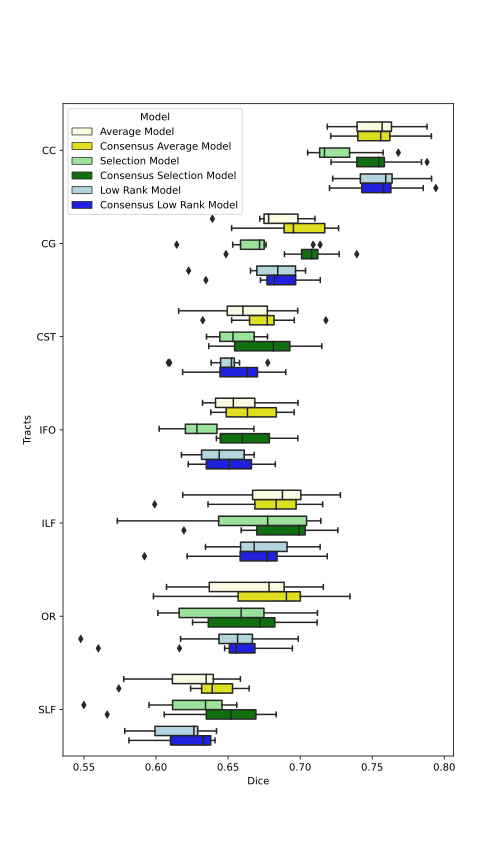
\includegraphics[width=\linewidth]{comparison-dice}
	\caption{Boxplots of the dice scores of all patients for all models. All
	subtracts are preprocessed seperatly, then merhed and the dice scores
are calculated for a binary mask of the joint subtracts.}
	\label{fig:Dice}
\end{figure}

\begin{table*}
\centering
\begin{tabular}{p{4cm}p{1.5cm}p{1cm}p{1cm}p{1cm}p{1cm}}
	{}  & \rot{Consensus   Average  Model} & \rot{Selection Model} &
	\rot{Consensus Selection Model} & \rot{Low Rank Model} & \rot{Consensus
	Low Rank Model} \\ \hline  
Average Model &   {\cellcolor{lightgreen} 0.001} & {\cellcolor{lightred} 0.001}
& {\cellcolor{lightgreen} 0.002} & {\cellcolor{lightred} 0.001} & 0.063 \\
Consensus Average Model &   & {\cellcolor{lightred} 0.001} & 0.900 &
{\cellcolor{lightred} 0.001} & {\cellcolor{lightred} 0.001} \\
Selection Model &    & & {\cellcolor{lightgreen} 0.001} & 0.900 & 0.494 \\
Consensus Selection Model &  &  &  & {\cellcolor{lightred} 0.001} &
{\cellcolor{lightred} 0.001} \\
Low Rank Model &   &
 &   & & 0.494 \\
\end{tabular}
\caption{Comparison of different models by Nemenyi post-hoc test. All $p$ values
below $0.05$ are marked. If the top model is significantly better in green else
in red.}
	\label{tab:sig}
\end{table*}


For a representative experiment we have reconstructed the corpus callosum (CC), the
cingulum (CG), the coricospinal tract (CST), the inferior fronto-occipital (IFO)
and the inferior longitudinal fasciculus (ILF), the optic radiation (OR), and
the superior longitudinal fasciculus (SLF). In the reference tragtographies, the
CC and SLF tracts were divided into subtracts, which we have merged into a single
tract. Further, we have merged the left and right parts of each tract. We have
evaluated the reconstruction quality by Dice score which is defined as
\[ 
	DICE = \frac{2 |RD \cap TR |}{|TR| + |RD|} ,
\]
where $RD$ denotes the reference data and $TR$ the tracking results
\cite{SCHILLING2019194}. A high Dice score is desired, as it denotes a high
overlap and a low overreach. To validate the results further, we applied a
Friedman test on model level to investigate if a model is significantly better
than any other model \cite{doi:10.1080/01621459.1937.10503522}. Post-hoc we
applied Nemenyi test to identify which models are significantly different
\cite{Nemenyi}.  


Figure \ref{fig:Dice} and Table \ref{tab:sig} summarize the results of our
quantitative comparison. In Fig. \ref{fig:Dice}, results from the average,
selection and low-rank model with and without use of the consensus model are
visualized using box plots to show the tract wise distribution of the Dice
scores. In Table \ref{tab:sig} the results of the post hoc Nemenyi tests are
shown. As a first result we denote that the Friedman test has shown that there
are significant differences between the models. 

To justify our previous work further, we are interested in the comparison of the
average, selection and low-rank model. The first impression from Fig.
\ref{fig:Dice} is that the average model is preferable to the other models and
that it depends on the tract if we prefer the selection or the low-rank model.
As it is visible in Table \ref{tab:sig} the improvement of the average model to
the other models is significant, while neither the selection model nor the
low-rank model is preferable to
the other. Therefore, we conclude that the average model, which we have proposed
within our last paper is significantly better than both other models. 

Within this work, we are more interested in the consensus model. Therefore, we
investigate if the improvement is significant between the model with and without
the application of the consensus. From Fig. \ref{fig:Dice} we can conclude, that
in 6 out of 7 tracts the consensus average model has an higher average Dice
score than the average model, that the consensus selection model has always an
higher Dice score, and that the consensus low-rank model has in 4 out of 7
tracts an higher Dice score. These changes are significant for the average and
selection model, while they are not significant for the low-rank model. 

Further, we want to compare the consensus models against each other. From Fig
\ref{fig:Dice} it seems that the consensus average and selection model are
preferable compared to the consensus low-rank model. Both models are equally
good compared by the mean dice score. This gets justified by the significance
tests. The consensus average as well as the consensus selection model are
significantly better than the consensus low-rank model. 

Overall we have shown that the consensus model improves our previously proposed
models significantly. However, the improvement by average Dice score is only for
the selection model large. 
\subsection{Computational Effort}
All experiments were computed on an Intel i9 with 3.3 GHz and 64 GB RAM. The
following durations are denoted in h:min:s or min:s.

The computation of a single bootstrap data sample took 1:10 on a single core,
multi-threaded fourth order fODF estimation took 4:33, the computation of the
selection model took 1:10, the computation of the averaging model took 1:30 and
the computation of the rank-3 model 0:40. The calculation of 100 bootstraps took
therefore 8:08:00, using all threads to create the bootstrap data as well as the
models. This also includes the computation of the consensus model, which on its
own took 11:00. The tracking itself is independent of the preprocessing steps.
It took approximately 3:30 for a bundle such it is shown in Figure
\ref{fig:Dice} on a single thread including postprocessing.  



\section{Conclusion}
\label{sec:conclusion}
Within this work we have evaluated the impact of measurement noise to the
average, selection and low-rank model. It has been shown, that the selection as
well as the average model are more resistant against noise than the low-rank
model. 
We have used the introduced uncertainty
to build a consensus model, which shows for the selection and average model
significantly better results compared to their base models. 
The highest increase in average Dice score is visible for the consensus
selection model compared to the base selection model. Compared to the average
model, the increasement is not that large, but significant. Together with the
huge computational effort, which is needed to create the consensus model
compared to the easieness of the base average model, we conclude that the
average model is able to increase the multi vector fields greatly at low cost
and is therefore, in almost all cases preferable. 

\section*{Acknowledgments}

We thank Gemma van der Voort (University of Bonn) for her initial proof-of-concept implementation of tractography with model averaging, and for providing feedback on our manuscript. This work was funded by the Deutsche Forschungsgemeinschaft (DFG, German Research Foundation) -- 422414649.
Data were provided by the Human Connectome Project, WU-Minn Consortium (Principal Investigators: David Van Essen and Kamil Ugurbil; 1U54MH091657) funded by the 16 NIH Institutes and Centers that support the NIH Blueprint
for Neuroscience Research; and by the McDonnell Center for Systems Neuroscience at Washington University.
\printbibliography
\end{document}
